\chapter{Analiza dziedziny problemu}
\label{cha:analizaDziedzinyProblemu}

%---------------------------------------------------------------------------

\section{Koncepcja cyfrowego zarządzania tożsamościami(IdM)}
\label{sec:konceptcjaIdM}

	Zarządzanie tożsamościami(Identity Management) jest podejściem do zagadnienia zapewnienia bezpieczeństwa dostępu do aplikacji w oparciu o dane identyfikujące użytkownika(Identity). Pojęcie danych identyfikujących może być zdefiniowane jako ,,informacje o jednostce pozwalające na identyfikację tej jednostki dla pewnej dziedziny zastosowań''\cite{Itu09}. W kontekście systemów zarządzania cyfrowymi tożsamościami dane identyfikujące mogą dotyczyć nie tylko osób ale również na przykład komponentów programowych\cite{Bertino11}. Zgodnie z rekomendacją Y.2720 w skład danych identyfikujących wchodzą identyfikator jednostki, dane uwierzytelniające jednostkę oraz atrybuty opisujące jednostkę\cite{Itu09}.

	Elisa Bertino i Kenji Takahashi w książce ,,Identity Management'' definiują cele zarządzania tożsamościami jako ,,utrzymanie integralności danych identyfikujących w trakcie ich użytkowania w celu udostępniania tych danych i powiązanych z nimi informacji w sposób bezpieczny i chroniący prywatność użytkowników''\cite{Bertino11}.
	 
	\subsection{Role w koncepcji systemów zarządzania tożsamościami}

		Systemy zarządzania tożsamościami charakteryzują się rozdzieleniem odpowiedzialności związanych z dostarczaniem funkcjonalności oraz zadań związanych z zapewnieniem bezpieczeństwa dostępu do aplikacji. Usługi uwierzytelniania i autoryzacji oraz funkcjonalności systemów dostarczane są dla jednostek - składowych systemu zarządzania tożsamościami - zazwyczaj użytkowników.
		Dane identyfikacyjne jednostek są gromadzone i wykorzystywane w trakcie korzystania z aplikacji. Dane osobowe mogą obejmować informacje związane z dokumentami tożsamości(numery dowodu osobistego, paszportu), dane bankowe, biometryczne oraz informacje związane z przebiegiem interakcji jednostki z systemem. Dane identyfikacyjne jednostek powinny być przetwarzane i gromadzone w sposób zapewniający  ochronę przed niewłaściwym użyciem. Nadużycia danych osobowych jednostek mogą prowadzić do istotnych strat użytkowników aplikacji.
		Elementem przeprowadzającym weryfikację tożsamości jednostek jest usługa ,,Identity Provider''(IdP). Usługa ta odpowiedzialna jest za przyporządkowywanie jednostkom atrybutów opisujących tożsamość, tworzenie powiązań pomiędzy różnymi atrybutami jednostki oraz tworzenie asercji zawierających informacje o atrybutach jednostek. 

		Usługa 'Identity Provider' może współpracować z innymi usługami tego typu dołączając do danych uwierzytelniających informacje udostępniane przez inne zaufane usługi IdP. Wykorzystanie danych uwierzytelniających dostarczanych przez inne usługi uwierzytelniające wymaga wprowadzenia procesu zapewnienia wiarygodności otrzymywanych danych. Proces ten może opierać się na przypisywaniu miary wiarygodności do atrybutów uwierzytelniających. Wyznaczenie wartości tej miary może być na przykład oparte o ocenę stopnia zaawansowania mechanizmów weryfikacji danych uwierzytelniających wykorzystywanych przez usługę dostarczająca dany atrybut tożsamości.

		Dostawcy usług wykorzystujący infrastrukturę systemów zarządzania tożsamościami przed zezwoleniem na dostęp do swoich zasobów zlecają usługom typu IdP przeprowadzenie procesu uwierzytelniania klienta na podstawie otrzymanych danych uwierzytelniających. Dostawcy usług powinni mieć możliwość deklaracji poziomu skuteczności zabezpieczeń wykorzystywanych w procesie autoryzacji dostępu do określonych zasobów. Poziom ten może być różny w zależności od rodzaju zasobu.

		Przedstawiona w książce ,,Identity Management Concepts, Technologies, and Systems'' terminologia wprowadza również pojęcie jednostki nadzorującej\cite{Bertino11}. Jest to najczęściej instytucja upoważniona prawnie do nadzoru nad procesami przetwarzania i przechowania danych osobowych lub wglądu  w informacje o charakterze poufnym.

	\subsection{Relacje miedzy rolami w systemach zarządzania tożsamościami}

		\begin{figure}[h]
			\centering
			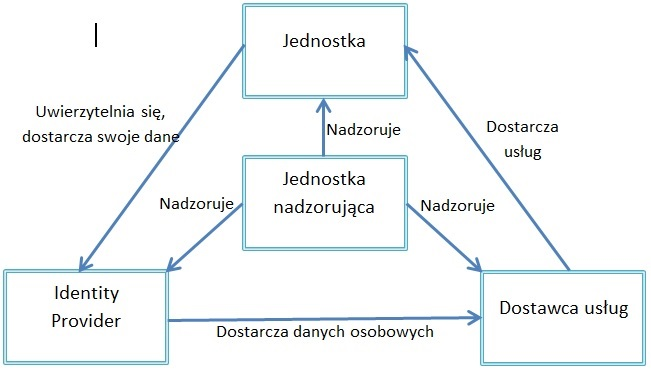
\includegraphics[width=15cm]{img/idmRelations.jpg}
			\caption{Relacje miedzy rolami w systemach zarządzania tożsamościami}
			\label{Relacje miedzy rolami w systemach zarządzania tożsamościami}
		\end{figure}

		Często stosowanym modelem jest infrastruktura złożona z jednej usługi typu ,,Identity Provider'' oraz wielu usług funkcjonalnych opierających na niej swoje mechanizmy zabezpieczeń. Dzięki takiemu rozwiązaniu dostawcy usług mogą skoncentrować się na tworzeniu funkcjonalności stanowiących istotę aplikacji - odpowiedzialności związane z zapewnieniem bezpieczeństwa dostępu delegowane są do usługi IdP. Specjalizowana usługa uwierzytelniania może dostarczać bardziej zaawansowanych zabezpieczeń. Dzięki realizacji tego modelu użytkownicy nie muszą zarządzać wieloma danymi uwierzytelniającymi dla różnych usług - dostęp do wielu serwisów gwarantowany jest przy użyciu tych samych danych. Wprowadza to jednak zagrożenia związane z centralizacja dostępu do różnych usług.

	\subsection{Federated Identity Management}

		Najczęściej użytkownicy korzystają nie z jednej usługi lecz z szerokiej gamy różnych usług. Każda z usług korzysta z własnych danych uwierzytelniających. Podejście ,,Federated Identity Management'' umożliwia tworzenie powiązań pomiędzy tożsamościami użytkownika w ramach różnych usług dzięki czemu dane uwierzytelniające każdej z sfederowanych usług mogą być wykorzystane w procesie uwierzytelniania dowolnej z usług.

	\subsection{Cykl życia tożsamości}

		Jednym z głównych zadań systemów zarządzania tożsamościami jest kontrola nad cyklem życia tożsamości. Autorzy książki ,,Identity Management: Concepts, Technologies and Systems'' opisują 4 etapy cyklu życiu tożsamości: tworzenie, użytkowanie, aktualizacja oraz wycofanie z użycia\cite{Bertino11}.

		Proces tworzenia cyfrowej tożsamości składa się z kilku kroków. Pierwszym z nich może być weryfikacja przedstawionych atrybutów tożsamości, wymagająca udowodnia przez jednostkę prawdziwości wprowadzanych danych. Następnie tworzone są dane uwierzytelniające. Ostatnim krokiem jest utworzenie tożsamości na podstawie otrzymanych danych oraz nadanie jednostce identyfikatora.

		Utworzona tożsamość może być wykorzystywana w różnych celach, np. zapewnienia wiarygodnej komunikacji lub w procesie jednokrotnego uwierzytelniania(ang. Single Sign-On).

		Systemy zarządzania tożsamościami powinny obsługiwać zmiany atrybutów tożsamości. Powinny aktualizować informacje o danych jednostek po zmianach wysyłając powiadomienia do usług przechowujących te dane, np. ,,Identity Provider''. Identyfikatory jednostek nie powinny podlegać zmianom. Systemy IdM muszą również usuwać tożsamości jeśli nie są już aktualne.

\section{Jednokrotne uwierzytelnianie}

	Książka ,,Identity Management: Concepts, Technologies and Systems'' definiuje jednokrotne uwierzytelnianie(ang. Single Sign-On) jako proces uwierzytelniania, w którym jednostka może wykorzystać wynik pojedynczego uwierzytelniania dla uzyskania dostępu do wielu niezależnych usług z ochroną dostępu\cite{Bertino11}. 

	Podstawą funkcjonowania mechanizmów jednokrotnego uwierzytelniania jest nawiązanie relacji zaufania pomiędzy dostawcami usług oraz serwisami typu ,,Identity Provider''. Po uwierzytelnieniu użytkownika w ramach jednej z usług objętych mechanizmem SSO dostęp do innej nie wymaga uwierzytelniania - dane uwierzytelniające są mapowane na dane niezbędne do uwierzytelnienia względem innej usługi oraz generowane są informacje pozwalające na uzyskanie dostępu do serwisu. Usługi korzystające z mechanizmu jednokrotnego uwierzytelniania powinny otrzymywać informacje kontekstowe o przebiegu procesu uwierzytelniania takie jak: wykorzystywane metody uwierzytelniania oraz sposób ochrony danych uwierzytelniających. Informacje te pozwalają na ocenę stopnia wiarygodności przeprowadzonego procesu uwierzytelniania.

	\subsubsection{Architektura systemów jednokrotnego uwierzytelniania}

		Implementacja mechanizmu jednokrotnego uwierzytelniania może opierać się o różne architektury. Autorzy książki ,,Identity Management: Concepts, Technologies and Systems''\cite{Bertino11} wymieniają następujące typy architektur systemów jednokrotnego uwierzytelniania:

		\begin{itemize}
		  \item Architektura oparta o brokery - architektura składająca się z punktu centralnego(serwera) oraz jednostek przez niego uwierzytelnianych. Serwer przydziela użytkownikom tokeny uwierzytelniające, dzięki którym możliwy jest dostęp do aplikacji. Przykładem architektury tego typu jest protokół Kerberos. 
		  \item Architektura oparta o agenty - architektura, w której w dostępie do każdej aplikacji pośredniczy agent uwierzytelniania. Jego rolą jest translacja pomiędzy metodą uwierzytelniania zastosowaną przez klienta a mechanizmami obsługiwanymi przez aplikację.
		  \item ,,Reverse proxy-based architecture'' - architektura wprowadzająca usługę proxy pośredniczącą w dostępie do wszystkich aplikacji objętych procedurą SSO. Moduł proxy dokonuje filtrowania przychodzących komunikatów - nieuwierzytelnione żądania zostają przekierowane, np. do serwera uwierzytelniającego.
		\end{itemize}
		  
		Procedura jednokrotnego uwierzytelniania pozwala na wygodniejszy sposób korzystania z aplikacji - znosi konieczność wielokrotnego wprowadzania danych identyfikujących. Użytkownik nie musi też zapamiętywać wielu haseł dla różnych usług. Wiele prostych haseł może zostać zastąpionych jedną bardziej wiarygodną metodą uwierzytelniania(np. z wykorzystaniem bardziej skomplikowanego hasła). Wadą wprowadzenia procedury jednokrotnego uwierzytelniania jest jednak centralizacja punktu dostępu do różnych aplikacji - złamanie zabezpieczeń otworzy drogę do wielu usług użytkownika.

%---------------------------------------------------------------------------

\section{Service-Oriented Architecture}
\label{sec:soa}

	Architektura zorientowana na usługi(ang. Service-Oriented Architecture) to architektura systemów informatycznych oparta o strukturę luźno powiązanych, rozproszonych usług, które mogą być wielokrotnie wykorzystywane i łączone w celu realizacji wymagań stawianych aplikacji. Architektura zorientowana na usługi umożliwia integrację usług w złożone procesy\cite{Lawler08}. Usługi składające się na architekturę SOA udostępniają swoje  funkcjonalności w ramach zdefiniowanych interfejsów i są od siebie niezależne. Komunikacja pomiędzy serwisami odbywa się poprzez wywołania dostarczanych przez nie operacji\cite{Papazoglou07}. 

	Architektura SOA zaprojektowana została jako rozwiązanie wielu problemów pojawiających się w trakcie tworzenia systemów rozproszonych. Do problemów tych należą: integracja aplikacji, zarządzanie transakcjami, zapewnienia bezpieczeństwa wykonywanych operacji, różnorodność środowisk uruchamiania aplikacji\cite{Papazoglou07}.

	Jednym z głównych założeń architektury zorientowanej na usługi jest niezależność od technologii implementacji. Jest to możliwe dzięki wykorzystaniu standardowych interfejsów usług oraz metod komunikacji pomiędzy nimi. Usługi w architekturze SOA są autonomiczne, same przechowują swój stan. W architekturze SOA wszelkie funkcjonalności są udostępniane w postaci usług.
	
	\subsection{Model architektury zorientowanej na usługi}
	
		Model architektury SOA definiuje charakterystyczne elementy architektury - komponenty, usługi i przetwarzanie informacji pomiędzy nimi - realizujące określone procesy biznesowe. Model ma budowę warstwową. Definicja warstw modelu ma na celu bardziej precyzyjne odwzorowanie pomiędzy wymaganiami biznesowymi, modelowaniem funkcjonalności a realizacją konkretnych rozwiązań dla stawianych wymagań.   	

	\subsection{Enterprise Service Bus} 

		W istniejących środowiskach dostarczania usług występuje często duża niejednorodność technologii, protokołów komunikacji i modeli wykorzystywanych przez różne serwisy. Jednym z rozwiązań tego problemu jest wprowadzenie warstwy pośredniczącej, która implementuje logikę pozwalającą na integrację różnorodnych usług. Rozwiązanie to stanowi podstawę dla koncepcji magistrali usług(ang. Enterprise Service Bus). 

		\begin{figure}[h]
			\centering
			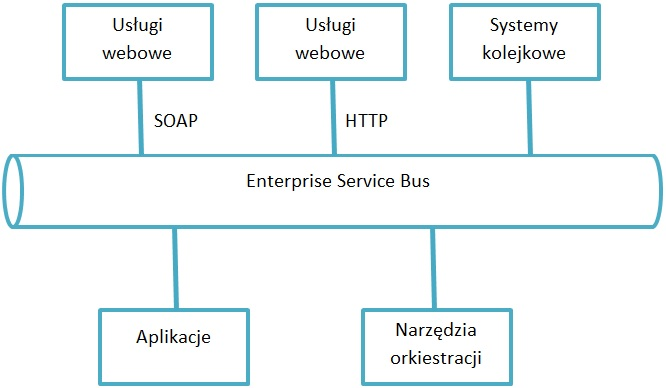
\includegraphics[width=15cm,height=8cm]{img/esb.jpg}
			\caption{Schemat funkcjonowania magistrali usług}
			\label{Schemat funkcjonowania magistrali uslug}
		\end{figure}

		Magistrala ESB dostarcza funkcjonalności rozproszonego przetwarzania oraz integracji usług opartych o standardowe mechanizmy. Funkcje transportu i transformacji wiadomości pozwalają na komunikację pomiędzy niejednorodnymi i rozproszonymi usługami. Magistrala usług może zapewniać mechanizmy bezpieczeństwa dostępu do aplikacji, wiarygodności dostarczania danych oraz audytu komunikacji. ESB powinno pozwalać na przekazywanie informacji kontekstowych np. dotyczących transakcji lub bezpieczeństwa dostępu do usług.

		Mechanizmy ESB uniezależniają klientów usług od fizycznych właściwości dostarczania usługi. Dzięki zastosowaniu magistrali usług możliwe jest dokonywanie zmian po stronie usługi lub zastąpienie usługi inną bez wpływu na aplikację kliencką. 

	\subsection{Zarządzanie procesami biznesowymi} 

		Istnieje szereg aplikacji, które realizując swoje funkcjonalności korzystają z różnorodnych usług. W ten sposób mogą powstawać skomplikowane procesy obejmujące komunikację z wieloma komponentami programowymi jak i interakcje z użytkownikami. Dla tego typu zastosowań użyteczne jest wprowadzenie mechanizmów zarządzania procesami biznesowymi(ang. Business Process Management) - technologii zapewniającej kontrolę nad przebiegiem wieloetapowych procesów obejmujących różne usługi w środowisku wielo-domenowym.

		Narzędzie zarządzania procesami biznesowymi pozwalają na automatyzację procesów. Definicja procesów opiera się o schemat organizacji zadań(ang. workflow). Narzędzie BPM umożliwiają wizualizację, modelowanie i analizę procesów biznesowych. Zarządzanie procesami biznesowymi jest dzięki temu metodologią pozwalającą na tworzenie, przedstawianie i nadzorowanie procesów biznesowych oraz upraszcza zrozumienie przebiegu procesu. Mechanizmy BPM pozwalają na monitorowania wykonania procesu biznesowego oraz dostęp do informacji o jego statusie. 

	\subsection{Zapewnienie bezpieczeństwa dostępu do usług w architekturze SOA}

		Ważnym aspektem dostarczania usług sieciowych jest zapewnienie mechanizmów bezpieczeństwa w procesie komunikacji. Mechanizmy bezpieczeństwa mogą być włączone w warstwie transportowej procesu dostarczania usług lub mogą być realizowane na poziomie wiadomości przesyłanej pomiędzy komunikującymi się jednostkami\cite{Szychowiak09}. 

		Zabezpieczenia warstwy transportowej polegają na zestawieniu szyfrowanej komunikacji pomiędzy klientem i dostawcą usług. Dzięki temu możliwe jest zapewnienie poufności wymiany wiadomości pomiędzy uczestnikami procesu komunikacji i integralności dostarczanych danych. Możliwa jest również implementacja mechanizmów uwierzytelniania w oparciu o szyfrowanie komunikatów\cite{Kolaczek09}.

		Istnieją sytuacje, w których zabezpieczenia warstwy transportowej nie są wystarczające.  Nie pozwalają one na zapewnienie bezpieczeństwa w razie konieczności przetwarzania informacji przez węzły pośrednie. Nie umożliwiają również zapewnienia poufności jedynie fragmentu wiadomości a nie całej jej treści. Rozwiązaniem tego problemów jest zastosowanie koncepcji mechanizmów bezpieczeństwa na poziomie przesyłanych wiadomości. Koncepcja ta zakłada oparcie mechanizmów bezpieczeństwa o informacje dołączane do wiadomości wymienianych pomiędzy klientem i dostawcą usługi. Przesyłane informacje mogą pozwalać na przeprowadzenie procesu uwierzytelniania lub zapewnienie integralności komunikatów. Istnieją liczne standardy opisujące format danych dołączanych do wiadomości oraz sposób ich przesyłania przy pomocy protokołów wykorzystywanych do dostarczania usług. Standardy tego typu definiują również sposób szyfrowania wymienianych wiadomości.		
%---------------------------------------------------------------------------

\section{Wymagania stawiane systemom Business-to-Business}
\label{sec:wymaganiaB2B}

Wymagania stawiane systemom Business-to-Business

%---------------------------------------------------------------------------

\section{Zakres wymagań tworzonego systemu}
\label{sec:zakresWymagan}

	W ramach projektu implementacyjnego  związanego z niniejszą pracą przygotowano przykłady ilustrujące zastosowanie mechanizmów systemów zarządzania tożsamościami. Punktem wyjścia była implementacja mechanizmu jednokrotnego uwierzytelniania oraz jednokrotnego wylogowywania dla aplikacji z interfejsem udostępnianym poprzez przeglądarkę internetową. Głównym celem projektu jest analiza mechanizmów zarządzania tożsamościami dla architektury zorientowanej na usługi.

	Przygotowywane moduły powinny korzystać z narzędzi uwierzytelniania i autoryzacji dostarczanych przez serwer aplikacyjny. Mechanizm uwierzytelniania powinien być oparty o protokół LDAP. Jako specyfikację realizującą założenia systemów zarządzania tożsamościami wybrano standard SAML opisany w dalszej części pracy.

	Najważniejszą częścią pracy było zastosowanie koncepcji systemów zarządzania tożsamościami w architekturze SOA. Praca powinna przedstawiać propozycję rozwiązania problemów uwierzytelniania i autoryzacji dostępu do usług sieciowych. W ramach projektu wymagana jest implementacja modułów wykorzystujących uwierzytelnianie oparte o mechanizmy systemów zarządzania tożsamościami dla różnych standardów dostarczania usług webowych(np. SOAP i REST). Należy również dokonać analizy zastosowania zaproponowanych mechanizmów uwierzytelniania w architekturze zorientowanej na usługi. Powinien zostać opracowany mechanizm magistrali usług pozwalający na przekazywanie informacji uwierzytelniających pomiędzy modułami systemu. Wykorzystanie zaimplementowanych usług wraz z mechanizmami zabezpieczania dostępu powinno być przedstawione w postaci modelu procesu biznesowego. 

	Dla ilustracji opisywanych mechanizmów opracowano zestaw usług dostarczających prostych funkcjonalności realizujących różne etapy dokonywania zamówienia w sklepie internetowym(usługi sprawdzania stanu magazynu, zlecenia wydania towaru,   zlecenia transportu, rejestracji transakcji w systemie finansowym). Usługi korzystają z uwierzytelniania w systemie zarządzania tożsamościami. Usługi zaimplementowane zostały przy użyciu różnych technologii.Unifikację sposobu korzystania z serwisów osiągnięto dzięki modułowi magistrali usług. Używając zaimplementowanych usług opracowano model procesu biznesowego realizujący kompletną funkcjonalność dokonywania zamówienia.
